\chapter{Imagens}
\label{chap:appendix}

\section{Visualizações específicas}

\begin{figure}[H]
    \centering
    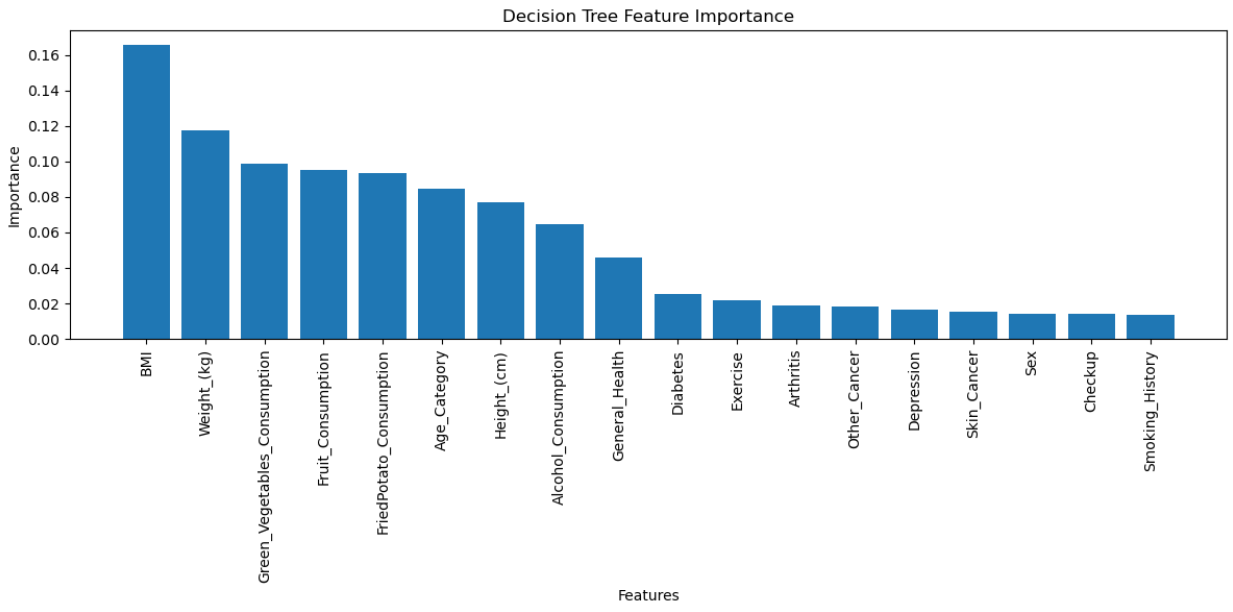
\includegraphics[width=0.9\textwidth]{images/feature_importance.png}
    \caption{\textit{Decision Trees}: Importância das variáveis identificadas pelo modelo.}
    \label{fig:feature_importance}
\end{figure}

\begin{figure}[H]
    \centering
    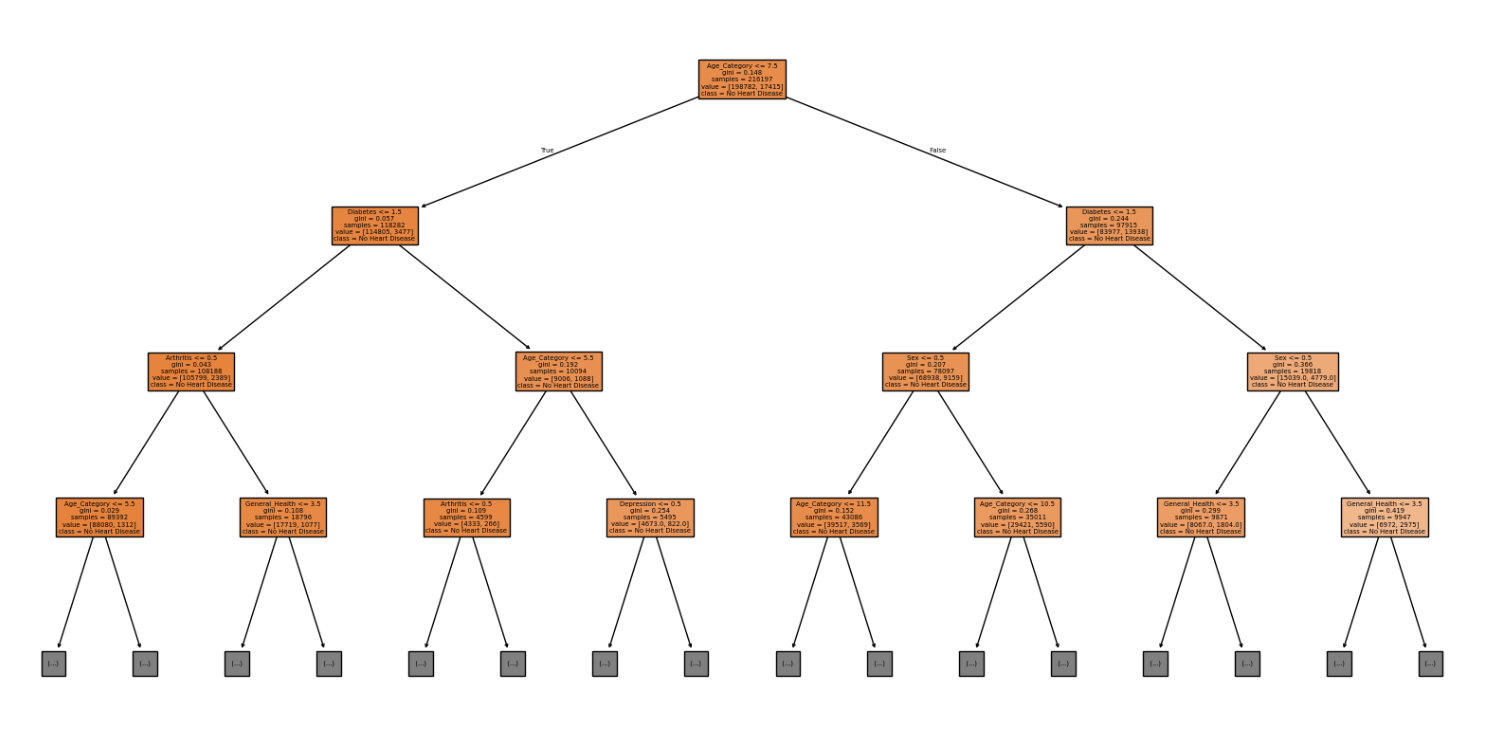
\includegraphics[width=0.9\textwidth]{images/decision_tree_structure.png}
    \caption{\textit{Decision Trees}: Visualização detalhada da estrutura da árvore gerada pelo modelo.}
    \label{fig:decision_tree_structure}
\end{figure}

\begin{figure}[H]
    \centering
    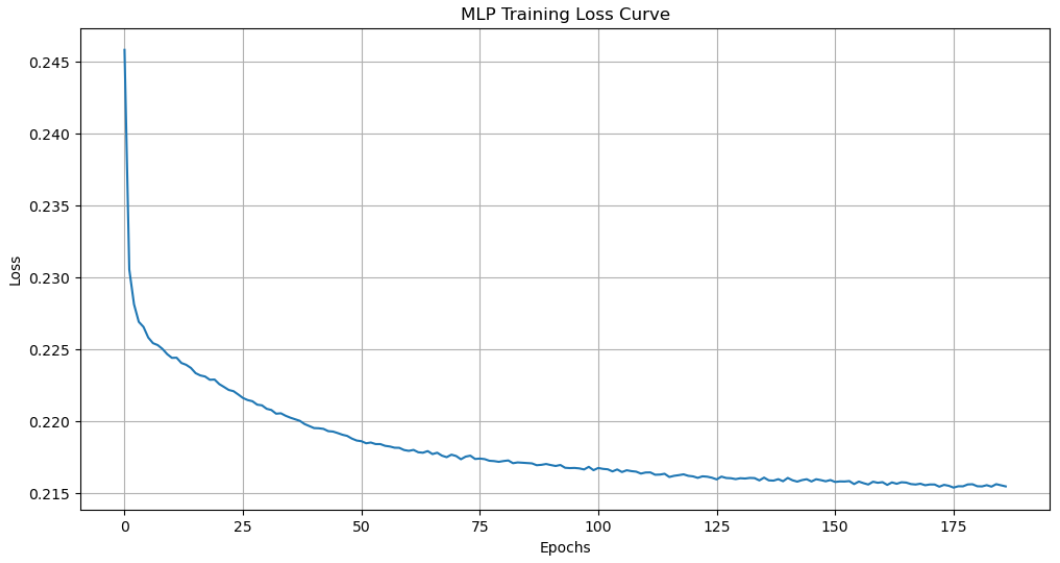
\includegraphics[width=0.9\textwidth]{images/mlp_training_loss.png}
    \caption{\textit{Multi-layer Perceptron}: Curva de perda durante o treino, mostrando a convergência do modelo.}
    \label{fig:mlp_training_loss}
\end{figure}

\begin{figure}[H]
    \centering
    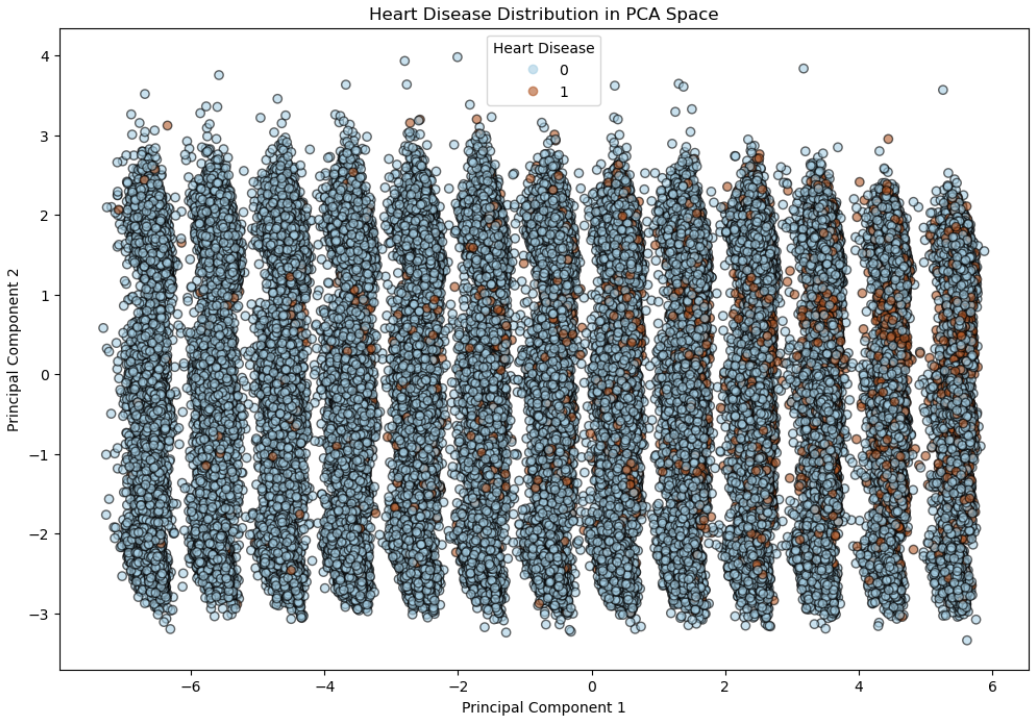
\includegraphics[width=0.9\textwidth]{images/knn_pca.png}
    \caption{\textit{k-NN}: Distribuição dos dados no espaço reduzido para 2 dimensões utilizando \textit{PCA}.}
    \label{fig:knn_pca}
\end{figure}

\section{Métricas individuais de modelos}
\begin{figure}[H]
    \centering
    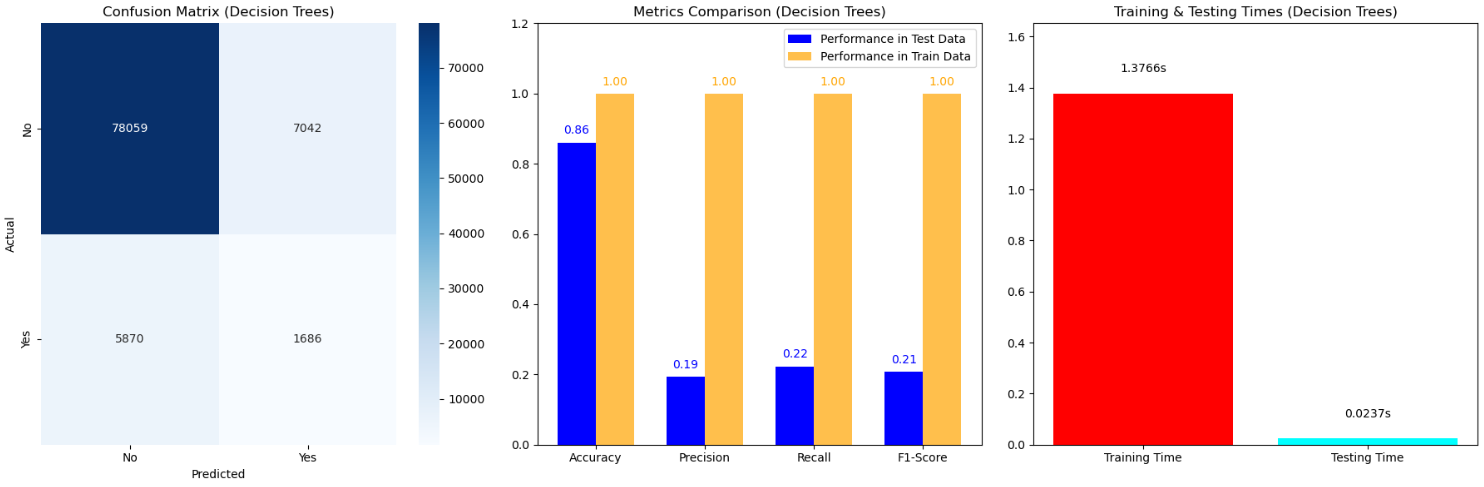
\includegraphics[width=0.9\textwidth]{images/decision_tree_overview.png}
    \caption{Modelo de \textit{Decision Trees}: Matriz de confusão, métricas de desempenho e tempos de execução.}
    \label{fig:decision_tree_overview}
\end{figure}

\begin{figure}[H]
    \centering
    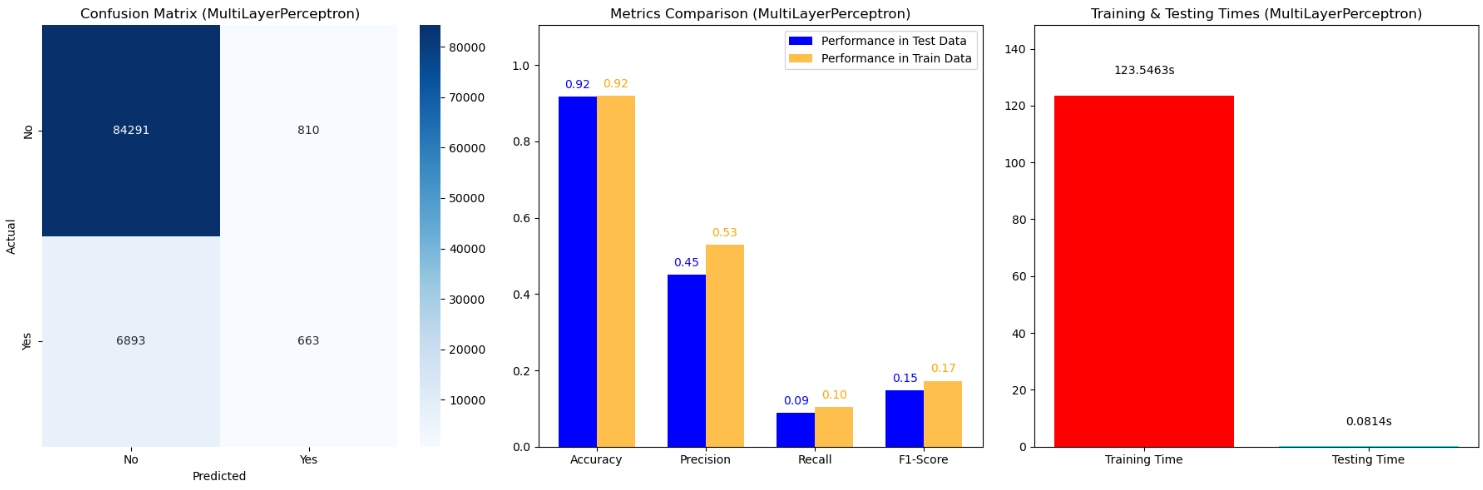
\includegraphics[width=0.9\textwidth]{images/mlp_overview.png}
    \caption{Modelo de \textit{Multi-layer Perceptron}: Matriz de confusão, métricas de desempenho e tempos de execução.}
    \label{fig:mlp_overview}
\end{figure}

\begin{figure}[H]
    \centering
    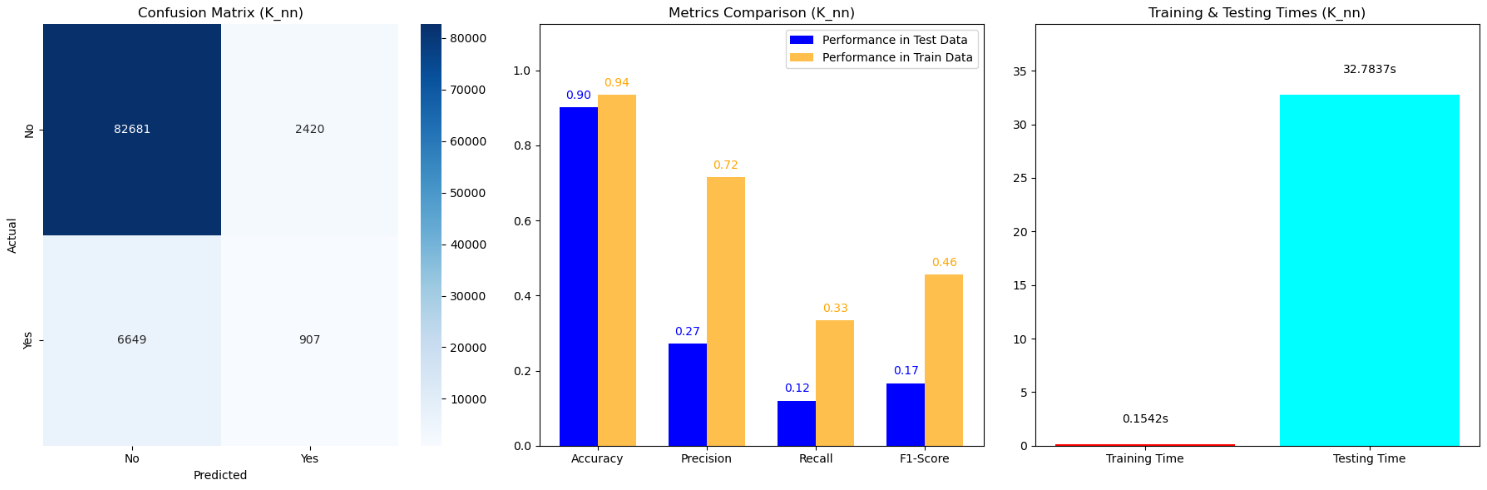
\includegraphics[width=0.9\textwidth]{images/knn_overview.png}
    \caption{Modelo de \textit{k-NN}: Matriz de confusão, métricas de desempenho e tempos de execução.}
    \label{fig:knn_overview}
\end{figure}

\section{Comparações}
\label{chap:comparacoes}

\begin{figure}[H]
    \centering
    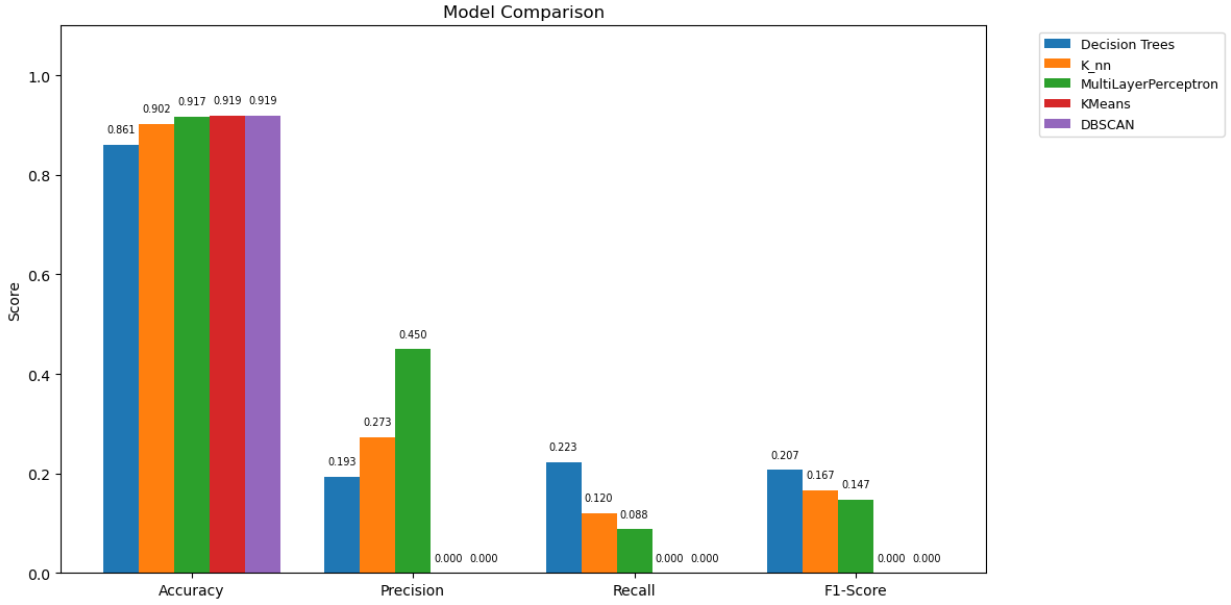
\includegraphics[width=0.9\textwidth]{images/model_comparison.png}
    \caption{Comparação geral do desempenho de todos os modelos.}
    \label{fig:model_comparison}
\end{figure}

\begin{figure}[H]
    \centering
    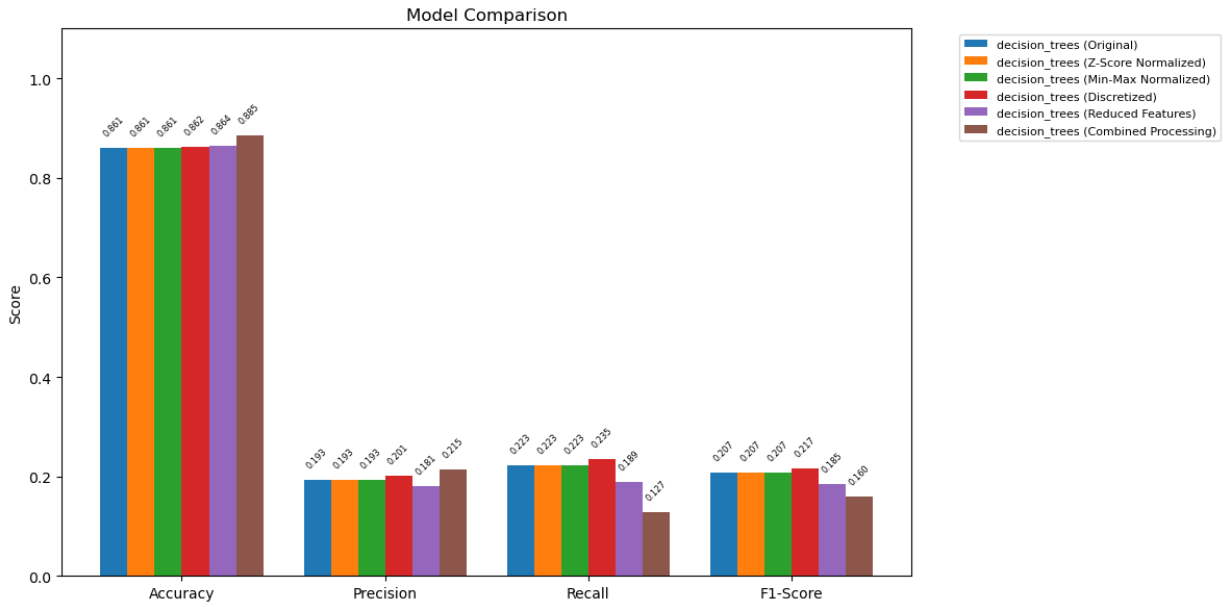
\includegraphics[width=0.9\textwidth]{images/decision_trees_comparison.png}
    \caption{\textit{Decision Trees}: Impacto de diferentes preparações dos dados no desempenho do modelo.}
    \label{fig:decision_trees_comparison}
\end{figure}

\begin{figure}[H]
    \centering
    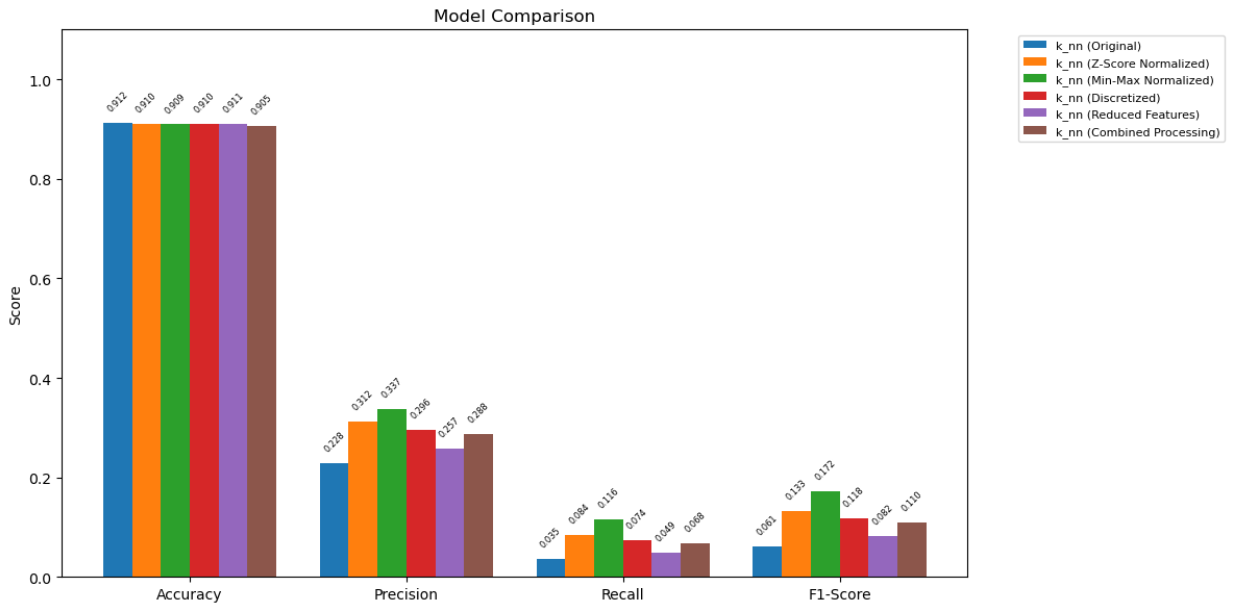
\includegraphics[width=0.9\textwidth]{images/knn_comparison.png}
    \caption{\textit{k-NN}: Impacto de diferentes preparações dos dados no desempenho do modelo.}
    \label{fig:knn_comparison}
\end{figure}

\begin{figure}[H]
    \centering
    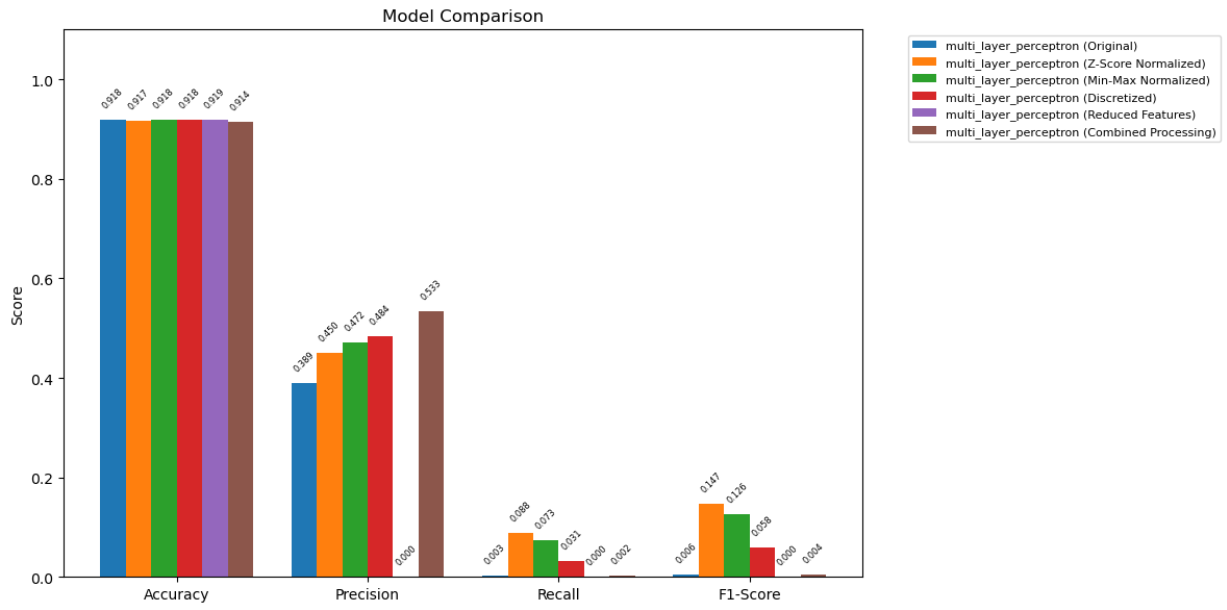
\includegraphics[width=0.9\textwidth]{images/mlp_comparison.png}
    \caption{\textit{Multi-layer Perceptron}: Impacto de diferentes preparações dos dados no desempenho do modelo.}
    \label{fig:mlp_comparison}
\end{figure}

